\documentclass[openany]{book}
\usepackage{lmodern}
\usepackage{amssymb,amsmath}
\usepackage{ifxetex,ifluatex}
\usepackage{fixltx2e} % provides \textsubscript
\ifnum 0\ifxetex 1\fi\ifluatex 1\fi=0 % if pdftex
  \usepackage[T1]{fontenc}
  \usepackage[utf8]{inputenc}
\else % if luatex or xelatex
  \ifxetex
    \usepackage{mathspec}
  \else
    \usepackage{fontspec}
  \fi
  \defaultfontfeatures{Ligatures=TeX,Scale=MatchLowercase}
\fi
% use upquote if available, for straight quotes in verbatim environments
\IfFileExists{upquote.sty}{\usepackage{upquote}}{}
% use microtype if available
\IfFileExists{microtype.sty}{%
\usepackage{microtype}
\UseMicrotypeSet[protrusion]{basicmath} % disable protrusion for tt fonts
}{}
\usepackage[margin=1in]{geometry}
\usepackage{hyperref}
\hypersetup{unicode=true,
            pdftitle={Spatial modelling of the electoral two-party preferred vote in Australia. A study of federal elections between 2001 and 2016 via the eechidna R package.},
            pdfauthor={Jeremy Forbes, Di Cook \& Rob Hyndman},
            pdfborder={0 0 0},
            breaklinks=true}
\urlstyle{same}  % don't use monospace font for urls
\usepackage{natbib}
\bibliographystyle{apalike}
\usepackage{longtable,booktabs}
\usepackage{graphicx,grffile}
\makeatletter
\def\maxwidth{\ifdim\Gin@nat@width>\linewidth\linewidth\else\Gin@nat@width\fi}
\def\maxheight{\ifdim\Gin@nat@height>\textheight\textheight\else\Gin@nat@height\fi}
\makeatother
% Scale images if necessary, so that they will not overflow the page
% margins by default, and it is still possible to overwrite the defaults
% using explicit options in \includegraphics[width, height, ...]{}
\setkeys{Gin}{width=\maxwidth,height=\maxheight,keepaspectratio}
\IfFileExists{parskip.sty}{%
\usepackage{parskip}
}{% else
\setlength{\parindent}{0pt}
\setlength{\parskip}{6pt plus 2pt minus 1pt}
}
\setlength{\emergencystretch}{3em}  % prevent overfull lines
\providecommand{\tightlist}{%
  \setlength{\itemsep}{0pt}\setlength{\parskip}{0pt}}
\setcounter{secnumdepth}{5}
% Redefines (sub)paragraphs to behave more like sections
\ifx\paragraph\undefined\else
\let\oldparagraph\paragraph
\renewcommand{\paragraph}[1]{\oldparagraph{#1}\mbox{}}
\fi
\ifx\subparagraph\undefined\else
\let\oldsubparagraph\subparagraph
\renewcommand{\subparagraph}[1]{\oldsubparagraph{#1}\mbox{}}
\fi

%%% Use protect on footnotes to avoid problems with footnotes in titles
\let\rmarkdownfootnote\footnote%
\def\footnote{\protect\rmarkdownfootnote}

%%% Change title format to be more compact
\usepackage{titling}

% Create subtitle command for use in maketitle
\newcommand{\subtitle}[1]{
  \posttitle{
    \begin{center}\large#1\end{center}
    }
}

\setlength{\droptitle}{-2em}

  \title{Spatial modelling of the electoral two-party preferred vote in Australia. A study of federal elections between 2001 and 2016 via the \texttt{eechidna} \texttt{R} package.}
    \pretitle{\vspace{\droptitle}\centering\huge}
  \posttitle{\par}
    \author{Jeremy Forbes, Di Cook \& Rob Hyndman}
    \preauthor{\centering\large\emph}
  \postauthor{\par}
      \predate{\centering\large\emph}
  \postdate{\par}
    \date{2019-03-26}

\usepackage{booktabs}
\usepackage{amsthm}
\makeatletter
\def\thm@space@setup{%
  \thm@preskip=8pt plus 2pt minus 4pt
  \thm@postskip=\thm@preskip
}
\makeatother
\usepackage{longtable}

\begin{document}
\maketitle

{
\setcounter{tocdepth}{1}
\tableofcontents
}
\hypertarget{intro}{%
\chapter{Introduction}\label{intro}}

Australia has changed in many ways over the last two decades. Rising house prices, country-wide improvements in education, an ageing population, and a decline in religious affiliation, are just a few facets of the country's evolving socio-demographic characteristics. At the same time, political power has moved back and forth between the two major parties. In the 2007 and 2010 federal elections, the Australian Labor Party (Labor) was victorious, whereas the 2001, 2004, 2013 and 2016 elections were won by the Liberal National coalition (Liberal). The two-party preferred vote, a measure of support between these two parties, fluctuated between 47.3\% and 53.5\% (in favour of the Liberal party) over this period. This study explores how electoral characteristics relate to two-party preference, and whether their effects have changed over time. Electoral socio-demographics are derived from the Census, and vote counts are obtained from federal elections.

Joining these two data sources is problematic as there in an inherent asynchronicity in the two events. A Census is conducted by the Australian Bureau of Statistics (ABS) every five years, whereas a federal election (conducted by the Australian Electoral Commission (AEC)) usually occurs every three years. The first problem addressed is that of obtaining appropriate Census data for the 2004, 2007, 2010 and 2013 elections - election years in which a Census does not occur. The predominant approach in previous studies is to join voting outcomes to the nearest Census, without accounting for any temporal differences (see \citet{DavisStimson98}, \citet{Stimson06}, \citet{Liao09} and \citet{Stimson09}). Furthermore, electoral boundaries change regularly, so spatial discrepancies also arise when matching electoral data. To obtain appropriate Census data for these four elections, electoral socio-demographics are imputed using a spatio-temporal imputation that combines areal interpolation \citep{Goodchild1993} and linear time-interpolation. Collecting and wrangling the raw data, along with the imputation process, are detailed in section \ref{data}. All data and associated documentation relating to this procedure are available in the \texttt{eechidna} \texttt{R} package \citep{eechidna}, providing a resource for future analysis .

Previous work on modelling Australian federal elections have found that aggregate socio-demographics are relatively good predictors of voting outcomes. \citet{Forrest01} does this using multiple regression of the Liberal and Labor primary vote for polling booths in the Farrer electorate in 1998. \citet{Stimson06}, \citet{Stimson09} and \citet{Stimson12} use principal component analysis of polling booths in the 2001, 2004 and 2007 elections respectively, also finding that socio-demographic characteristics of polling booths are linked to their two-party preferred vote. On the contrary, \citet{Stimson09} models the polling booth swing vote (change in the two-party preferred vote) in the 2007 election, finding that little of swing vote can be explained by Census data. Instead of analyzing a single election in isolation, this paper employs a consistent model framework across six elections so that temporal changes in the effects of socio-demographics can be observed, where each federal elections is modelled with a cross-sectional data set. The use of a regression framework to examine these socio-political relationships over time is seemingly absent from previous Australian studies. It also appears that no study has attempted any type of statistical analysis of socio-demographics in conjunction with voter behaviour in Australia since 2007, making this paper distinctly different from those previous.

The cross-sectional data set for each election consists of the two-party preferred vote (response variable), and socio-demographic variables (explanatory variables) that characterise each electorate. To obtain these cross-sections, socio-demographic variables are first standardized, and then principal components are used to group variables into ``factors''. To account for the inherent spatial structure of the data, a spatial error model is fit for each election. These steps are discussed in section \ref{modelling}. In section \ref{results} inference is conducted on the models to see which effects are significant, how effects change over time and which electorates have abnormal voting behaviour.

\hypertarget{data}{%
\chapter{Data collection, wrangling and imputation}\label{data}}

\hypertarget{collecting-the-data}{%
\section{Collecting the data}\label{collecting-the-data}}

The voting outcome of interest is the electoral two-party preferred vote, which is provided by the Australian Electoral Commission (AEC) for the 2001, 2004, 2007, 2010, 2013 and 2016 elections via the AEC Tally Room. The AEC divide Australia into 150 regions called electorates, with each corresponding to a single seat in the House of Representatives. Voting is compulsory in Australia, and each voter assigns a numbered preference to each available candidate in their electorate. The two-party preferred vote is determined by a tally of these preferences where, by convention, only the ranks of the Labor and Liberal candidates are considered. This is recorded as a percentage preference in favour of the Liberal party.

Socio-demographic variables are derived from the Census of Population and Housing (Census), which is a survey of every household in Australia, recording information such as age, gender, ethnicity, education level and income. There have been four Censuses in the 21st century, being that in 2001, 2006, 2011 and 2016. The Australian Bureau of Statistics (ABS) conducts the Census and publishes aggregated information. The ABS approximation of electorates at the time of the Census is chosen. From this aggregate information, 67 socio-demographic variables are computed for each of the electorates.

Raw data is sourced online from the AEC and ABS websites in .csv and .xlsx files. The format of these files change over the years, making extracting the appropriate information a big task. The functions available in the \texttt{dplyr} \citep{dplyr} and \texttt{readxl} \citep{readxl} \texttt{R} packages are very useful, as they provide fast consistent tools for data manipulation and functions to import .xlsx files (respectively). The 2001 and 2006 Census data are however published in a format where each electorate has a separate document, making it difficult to use the \texttt{dplyr} tools and instead cells have to be selected from each individual file to construct the desired variables. All scripts required for the data wrangling process can be found in the github repository for the \texttt{eechidna} \texttt{R} package \citep{eechidna}, along with the raw data. The \texttt{eechidna} package makes this study entirely reproducible and provides a resource to help wrangle data for future Censuses and elections, when they become available.

\hypertarget{joining-census-and-election-data}{%
\section{Joining Census and election data}\label{joining-census-and-election-data}}

\hypertarget{differences-between-census-and-election-data}{%
\subsection{Differences between Census and election data}\label{differences-between-census-and-election-data}}

Between 2001 and 2016 there were six elections and four Censuses (see Figure \ref{fig:timeline}). Electoral boundaries are redistributed regularly by the AEC, meaning that only in the years where both a Census and election occur will the boundaries match - the case for the 2001 and 2016 election. Therefore, for the four elections between 2004 and 2013, both temporal and spatial differences in electorates need to be accounted for when joining the electoral two-party preferred vote with Census data. For these elections a spatio-temporal imputation method is employed to obtain electoral socio-demographics. This method uses Census information from both before and after the election of interest.

\begin{figure}[h]

{\centering 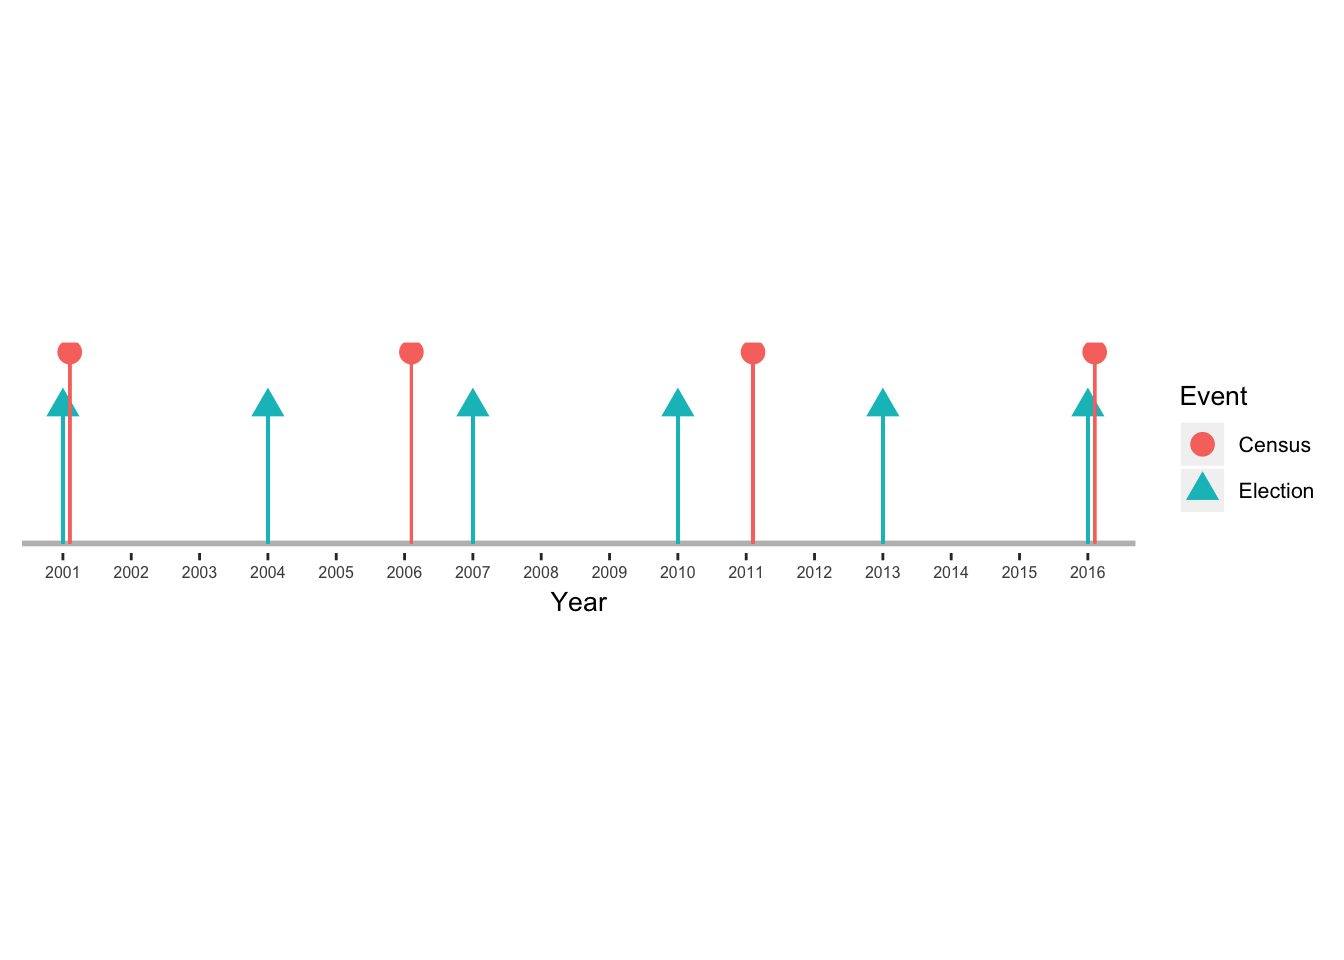
\includegraphics[width=0.9\linewidth]{electoral-modelling-draft_files/figure-latex/timeline-1} 

}

\caption{Timeline of Australian elections and Censuses. They do not always occur in the same year.}\label{fig:timeline}
\end{figure}

\hypertarget{spatio-temporal-imputation}{%
\subsection{Spatio-temporal imputation}\label{spatio-temporal-imputation}}

To account for spatial differences, the piece-wise approximation method in \citet{Goodchild1993} is adopted. Consider a map of source zones \(s = 1,...,S\), for which socio-demographic information is available, and a set of target zones \(t = 1,...,T\) for which information is to be imputed. In this context the map of electoral boundaries at the time of a Census would be the source zones, and the boundaries at the time of the election would be the target zones. Denote the area of intersection between source zone \(s\) and target zone \(t\) as \(A_{s,t}\), the population of the source zone \(s\) as \(U_s\), and the population of intersection between source zone \(s\) and target zone \(t\) as \(P_{s,t}\).

Compute each \(A_{s,t}\) and estimate population of the intersection:

\[\hat{P}_{s,t} = \frac{U_s*A_{s,t}}{\sum_{t=1}^T A_{s,t}}\]
This assumes that populations are uniformly distributed within each source zone.

In order to calculate socio-demographic information for each of the target zones, a weighted average is taken using the estimated population as weights. Denote a given Census variable for the target zone \(C_t\), and the same Census variable for the source zone \(D_s\):

\[\hat{C}_t = \frac{\sum_{s=1}^{S}{D_s*\hat{P}_{s,t}}}{\sum_{s=1}^{S}{\hat{P}_{s,t}}}\]
This assumes that each individual in a source zone assumes the aggregate characteristics of the zone.

Applying this to each of the target zones addresses the spatial component, as it imputes the required socio-demographic for the desired electoral boundaries. However these are applicable at the time of the Census (source year) and are not yet appropriate for the election (target year).

Denote year \(y\), with a Census falling on \(y_1\) and \(y_3\), and an election on year \(y_2\), and add this subscript to the Census variable estimate, \(\hat{C}_{t,y}\). To account for temporal changes, linear interpolation is used between Census years to get the final estimate of a Census variable for the target zone in the election year \(y_2\). This assumes that population evolves in a linear manner over time.

\[\hat{C}_{t,y_2} = \frac{y_3-y_2}{y_3-y_1}*\hat{C}_{t,y_1} + \frac{y_2-y_1}{y_3-y_1}*\hat{C}_{t,y_3}\]

\hypertarget{applied}{%
\subsection{Applied}\label{applied}}

Publically available Census data is aggregated and there are different resolutions accessible, ranging from SA1 (over 50,000 zones) to electoral divisions (150 zones). For this study electoral divisions are used as source zones, and this imputation method is applied for each of the 2004, 2007, 2010 and 2013 elections. To demonstrate its functionality, consider the imputation of socio-demographic variables for the electorate of Hume in New South Wales (NSW), at the time of the 2013 federal election. Figure \ref{fig:hume13} shows this region amongst other NSW electorates.

\begin{figure}[h]

{\centering 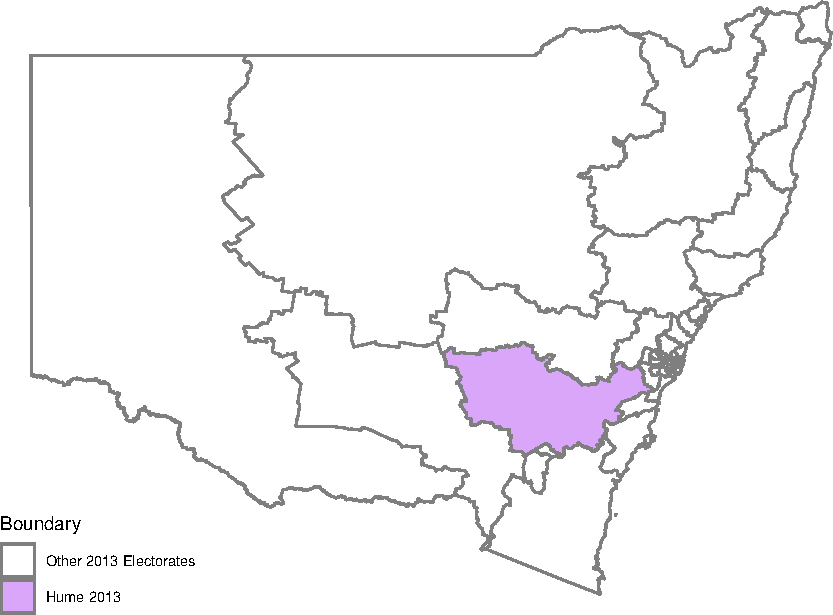
\includegraphics[height=0.3\textheight]{electoral-modelling-draft_files/figure-latex/hume13-1} 

}

\caption{Some of the electoral boundaries in NSW for 2013, with the electoral boundary for Hume, shown in purple.}\label{fig:hume13}
\end{figure}

The Censuses neighbouring the 2013 election are those in 2011 and 2016, and the Hume boundary is changed, as seen by plotting the Hume boundary (purple) in the 2013 election over the divisions in 2016 (see Figure \ref{fig:hume16}).

\begin{figure}[h]

{\centering 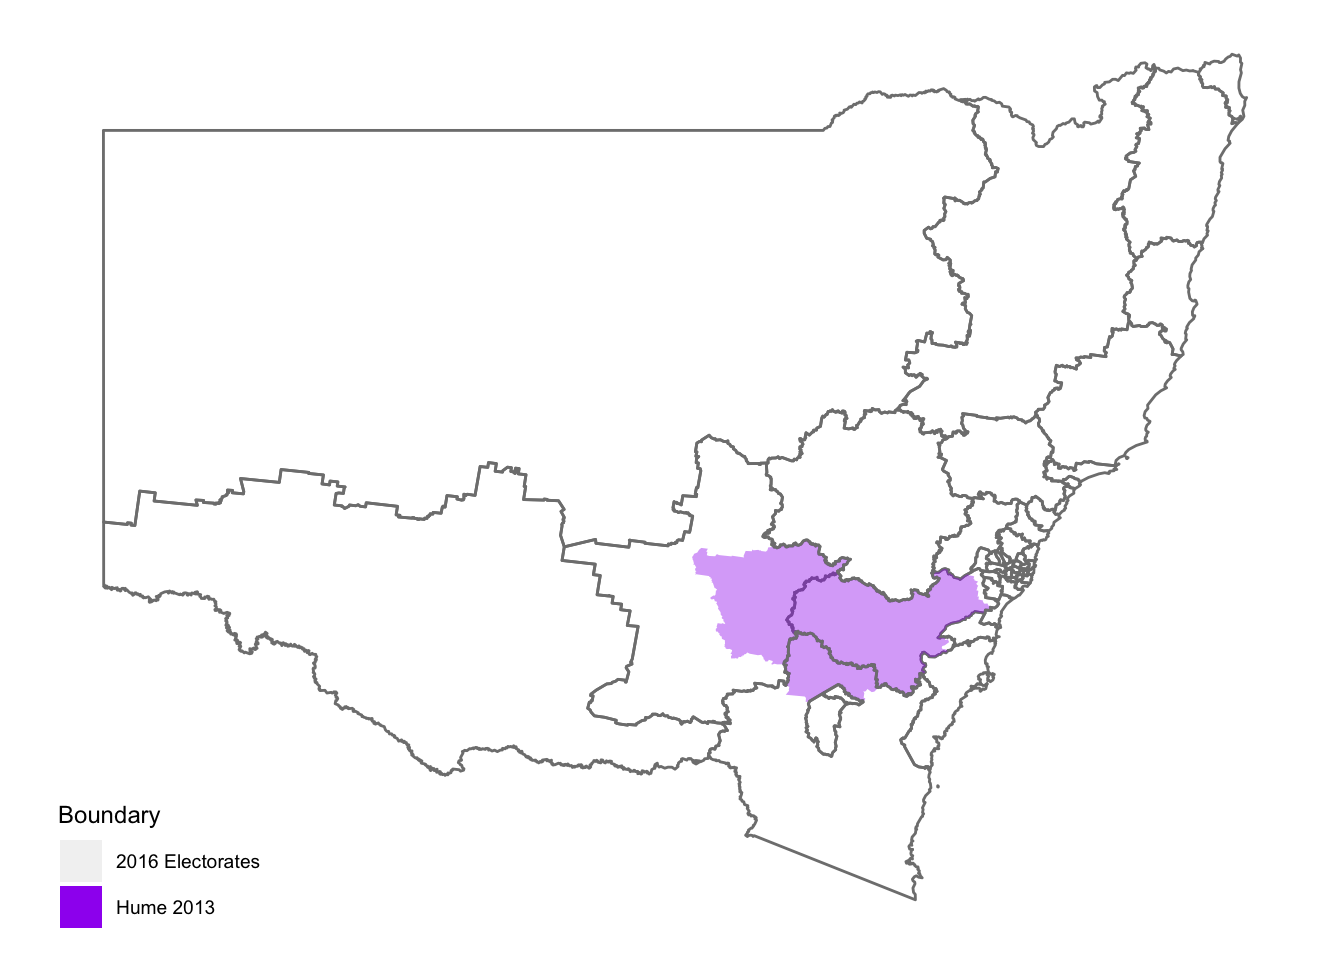
\includegraphics[height=0.3\textheight]{electoral-modelling-draft_files/figure-latex/hume16-1} 

}

\caption{Census division boundaries in NSW for 2016, with the 2013 electoral boundary for Hume, shown in purple. The purple region is not contained within a single Census division.}\label{fig:hume16}
\end{figure}

There are many electorates in 2016 that intersect with the purple region (Hume boundary for 2013), these include the divisions of Riverina, Eden-Monaro and Hume, along with smaller intersecting areas with Fenner, Calare, Gilmore and Whitlam. To impute Census information for this purple region, calculate the percentage of each 2016 electorate that intersects with the purple region, which is then used to estimate intersection populations \(\hat{P}_{s,t}\).

\begin{longtable}[]{@{}llll@{}}
\toprule
\begin{minipage}[b]{0.17\columnwidth}\raggedright
Electorate (2016)\strut
\end{minipage} & \begin{minipage}[b]{0.10\columnwidth}\raggedright
Percentage\strut
\end{minipage} & \begin{minipage}[b]{0.22\columnwidth}\raggedright
Population in Electorate\strut
\end{minipage} & \begin{minipage}[b]{0.40\columnwidth}\raggedright
Estimated Population Allocated to Purple Region: \(\hat{P}_{s,t}\)\strut
\end{minipage}\tabularnewline
\midrule
\endhead
\begin{minipage}[t]{0.17\columnwidth}\raggedright
HUME\strut
\end{minipage} & \begin{minipage}[t]{0.10\columnwidth}\raggedright
96.54\%\strut
\end{minipage} & \begin{minipage}[t]{0.22\columnwidth}\raggedright
150643\strut
\end{minipage} & \begin{minipage}[t]{0.40\columnwidth}\raggedright
145427\strut
\end{minipage}\tabularnewline
\begin{minipage}[t]{0.17\columnwidth}\raggedright
RIVERINA\strut
\end{minipage} & \begin{minipage}[t]{0.10\columnwidth}\raggedright
25.11\%\strut
\end{minipage} & \begin{minipage}[t]{0.22\columnwidth}\raggedright
155793\strut
\end{minipage} & \begin{minipage}[t]{0.40\columnwidth}\raggedright
39117\strut
\end{minipage}\tabularnewline
\begin{minipage}[t]{0.17\columnwidth}\raggedright
EDEN-MONARO\strut
\end{minipage} & \begin{minipage}[t]{0.10\columnwidth}\raggedright
11.09\%\strut
\end{minipage} & \begin{minipage}[t]{0.22\columnwidth}\raggedright
147532\strut
\end{minipage} & \begin{minipage}[t]{0.40\columnwidth}\raggedright
16358\strut
\end{minipage}\tabularnewline
\begin{minipage}[t]{0.17\columnwidth}\raggedright
CANBERRA\strut
\end{minipage} & \begin{minipage}[t]{0.10\columnwidth}\raggedright
0.28\%\strut
\end{minipage} & \begin{minipage}[t]{0.22\columnwidth}\raggedright
196037\strut
\end{minipage} & \begin{minipage}[t]{0.40\columnwidth}\raggedright
548\strut
\end{minipage}\tabularnewline
\begin{minipage}[t]{0.17\columnwidth}\raggedright
FENNER\strut
\end{minipage} & \begin{minipage}[t]{0.10\columnwidth}\raggedright
0.23\%\strut
\end{minipage} & \begin{minipage}[t]{0.22\columnwidth}\raggedright
202955\strut
\end{minipage} & \begin{minipage}[t]{0.40\columnwidth}\raggedright
474\strut
\end{minipage}\tabularnewline
\begin{minipage}[t]{0.17\columnwidth}\raggedright
WHITLAM\strut
\end{minipage} & \begin{minipage}[t]{0.10\columnwidth}\raggedright
0.06\%\strut
\end{minipage} & \begin{minipage}[t]{0.22\columnwidth}\raggedright
152280\strut
\end{minipage} & \begin{minipage}[t]{0.40\columnwidth}\raggedright
92\strut
\end{minipage}\tabularnewline
\begin{minipage}[t]{0.17\columnwidth}\raggedright
GILMORE\strut
\end{minipage} & \begin{minipage}[t]{0.10\columnwidth}\raggedright
0.06\%\strut
\end{minipage} & \begin{minipage}[t]{0.22\columnwidth}\raggedright
150436\strut
\end{minipage} & \begin{minipage}[t]{0.40\columnwidth}\raggedright
86\strut
\end{minipage}\tabularnewline
\begin{minipage}[t]{0.17\columnwidth}\raggedright
CALARE\strut
\end{minipage} & \begin{minipage}[t]{0.10\columnwidth}\raggedright
0.01\%\strut
\end{minipage} & \begin{minipage}[t]{0.22\columnwidth}\raggedright
161298\strut
\end{minipage} & \begin{minipage}[t]{0.40\columnwidth}\raggedright
21\strut
\end{minipage}\tabularnewline
\bottomrule
\end{longtable}

Now consider the socio-demographic \(AusCitizen\) - the proportion of people in the region who are Australian citizens.

\begin{longtable}[]{@{}lll@{}}
\toprule
\begin{minipage}[b]{0.18\columnwidth}\raggedright
DivisionNm\strut
\end{minipage} & \begin{minipage}[b]{0.21\columnwidth}\raggedright
AusCitizen (\%): \(D_s\)\strut
\end{minipage} & \begin{minipage}[b]{0.53\columnwidth}\raggedright
Estimated Population Allocated to Purple Region: \(\hat{P}_{s,t}\)\strut
\end{minipage}\tabularnewline
\midrule
\endhead
\begin{minipage}[t]{0.18\columnwidth}\raggedright
HUME\strut
\end{minipage} & \begin{minipage}[t]{0.21\columnwidth}\raggedright
90.02\strut
\end{minipage} & \begin{minipage}[t]{0.53\columnwidth}\raggedright
145427\strut
\end{minipage}\tabularnewline
\begin{minipage}[t]{0.18\columnwidth}\raggedright
RIVERINA\strut
\end{minipage} & \begin{minipage}[t]{0.21\columnwidth}\raggedright
89.11\strut
\end{minipage} & \begin{minipage}[t]{0.53\columnwidth}\raggedright
39117\strut
\end{minipage}\tabularnewline
\begin{minipage}[t]{0.18\columnwidth}\raggedright
EDEN-MONARO\strut
\end{minipage} & \begin{minipage}[t]{0.21\columnwidth}\raggedright
88.00\strut
\end{minipage} & \begin{minipage}[t]{0.53\columnwidth}\raggedright
16358\strut
\end{minipage}\tabularnewline
\begin{minipage}[t]{0.18\columnwidth}\raggedright
CANBERRA\strut
\end{minipage} & \begin{minipage}[t]{0.21\columnwidth}\raggedright
85.48\strut
\end{minipage} & \begin{minipage}[t]{0.53\columnwidth}\raggedright
548\strut
\end{minipage}\tabularnewline
\begin{minipage}[t]{0.18\columnwidth}\raggedright
FENNER\strut
\end{minipage} & \begin{minipage}[t]{0.21\columnwidth}\raggedright
83.64\strut
\end{minipage} & \begin{minipage}[t]{0.53\columnwidth}\raggedright
474\strut
\end{minipage}\tabularnewline
\begin{minipage}[t]{0.18\columnwidth}\raggedright
WHITLAM\strut
\end{minipage} & \begin{minipage}[t]{0.21\columnwidth}\raggedright
89.52\strut
\end{minipage} & \begin{minipage}[t]{0.53\columnwidth}\raggedright
92\strut
\end{minipage}\tabularnewline
\begin{minipage}[t]{0.18\columnwidth}\raggedright
GILMORE\strut
\end{minipage} & \begin{minipage}[t]{0.21\columnwidth}\raggedright
89.03\strut
\end{minipage} & \begin{minipage}[t]{0.53\columnwidth}\raggedright
86\strut
\end{minipage}\tabularnewline
\begin{minipage}[t]{0.18\columnwidth}\raggedright
CALARE\strut
\end{minipage} & \begin{minipage}[t]{0.21\columnwidth}\raggedright
87.56\strut
\end{minipage} & \begin{minipage}[t]{0.53\columnwidth}\raggedright
21\strut
\end{minipage}\tabularnewline
\bottomrule
\end{longtable}

Then taking a weighted average of \(AusCitizen\) using the estimated population as weights yields \(\hat{C}_{Hume,2016} = 89.65 \%\). Repeating this process using the 2011 Census and electoral boundaries yields \(\hat{C}_{Hume,2011} = 91.00 \%\)

Finally, linearly interpolate between 2011 and 2016 to arrive at the 2013 estimate:
\begin{eqnarray*}
\hat{C}_{Hume,2013} & = &\frac{3}{5} \cdot \hat{C}_{Hume,2011} + \frac{2}{5} \cdot \hat{C}_{Hume,2016} \\ 
& = & \frac{3}{5} \cdot 91.00 \% + \frac{2}{5} \cdot 89.65 \% \\ 
& = & 90.46 \%
\end{eqnarray*}

This is done for each of the socio-demographic variables, and repeated each of the 2013 electorates.

\hypertarget{modelling}{%
\chapter{Modelling}\label{modelling}}

\hypertarget{data-pre-processing}{%
\section{Data pre-processing}\label{data-pre-processing}}

With socio-demographic information now available for each electorate, each election is joined to the data corresponding with its two-party preferred vote. Socio-demographic variables within each election year are standardized to have mean zero and variance one, to adjust for changing variable scales. For example, inflation-adjusted median rental prices increased across almost all electorates, with median rent of 200 dollars per week placing an electorate in the 90th percentile in 2001, but only the 30th percentile in 2016.

\hypertarget{dimension-reduction}{%
\subsection{Dimension reduction}\label{dimension-reduction}}

With only \(N = 150\) observations (electorates) in each election and \(p = 65\) socio-demographic variables in each cross-section, any model using all variables would face serious problems with multi-collinearity and over-fitting, likely leading to erroneous conclusions regarding variable significance. Therefore a form of dimension reduction is adopted before models are fit.

Socio-demographic variables\footnote{A preliminary step involved removing all age bands, because age is represented by median age, and to remove variables relating to particular denominations of Christianity.} that represent similar information are combined into ``factors'' using principal component analysis (PCA). The scree plots of the principal components for each election all level off after four components, and the loadings of these four components are similar across the elections. Principal components are then computed on the combined set of socio-demographics across all six elections. A factor is created by combining several variables all have large loadings in a particular component and when there is an intuitive reason as to why these variables could represent common information. A loading with magnitude greater than 0.15 is considered large. After computing these sums, each factor is again standardized to have mean zero and variance one, within each election.

Consider the \texttt{Incomes} factor as an illustration. Independent of principal components, we may suspect that median personal income, median household income and median family income are providing similar information about the financial wellbeing of an electorate. Their loadings in the first principal component are large (0.20, 0.21 and 0.22 respectively), which provides the evidence needed to combine these variables into a single factor, which is called \texttt{Incomes}.

This process reduces the predictor set to \(p = 30\).

\hypertarget{model-framework}{%
\section{Model framework}\label{model-framework}}

An identical model specification is used across the six elections, with each election modelled separately. This allows for the socio-demographic effects to be estimated separately for each year, allowing for interpretation of temporal changes in these effects. This is preferable over a single longitudinal model because it avoids any concerns of undue bias stemming from an incorrectly imposed time-varying restriction on any variable. Without such restrictions, a pooled cross-sectional model does not yield any distinct advantage over separate cross-sections. The panel approach is avoided because of how frequently electoral boundaries change, meaning that electorates that have the same name across elections are not guaranteed to represent the same geographical region. Therefore any fixed or random effects models would be difficult to estimate without implementing consistent boundaries, which would requiring further imputation.

For each cross-section, let the response variable be the two-party preferred vote in favour of the Liberal party, denoted \(Y\), with \(Y = 70\) representing a 70\% preference for Liberal, 30\% for Labor. Although \(Y\) lies in the interval \((0,100)\), observed values are never very close to 0 or 100 (minimum \(24.05 \%\) and maximum \(74.90 \%\)), so there is no need to impose the constraint of \(Y \in [0,100]\). Furthermore, the response is found to be spatially correlated in each election (Moran's I test, \(p \le 7\cdot10^{-15}\)). This is expected, as electorates are aggregate spatial units, and hence the spatial structure of the data must modelled appropriately.

The spatial error model \citep{Anselin88} is chosen because captures spatial heterogeneity by incorporating a spatially structured random effect vector \citep{LeSage2009}. In this context, the random effect can be thought of as capturing the unobserved political climate in each electorate, where the climate is correlated with the climate in neighbouring electorates. This functions under the assumption that the climate is independent of electoral socio-demographics, and that an electorate is equally correlated with any electorate that shares a part of its boundary. Spatial weights are calculated in accordance with these assumptions. The spatial error model is specified as follows:

Let \(\rho\) be spatial autoregressive coefficient, \(\boldsymbol v\) be a spherical error term, \({\boldsymbol W}\) be a matrix of spatial weights (containing information about the neighbouring regions), \(\boldsymbol X\) be a matrix of socio-demographic covariates, \(\boldsymbol \beta\) be a vector of regression coefficients and \(\boldsymbol a\) be a spatially structured random effect vector.

\[{\boldsymbol y} = {\boldsymbol X} {\boldsymbol \beta} + {\boldsymbol a}\]
and

\[{\boldsymbol a} = \rho {\boldsymbol W} {\boldsymbol a} + {\boldsymbol v}\]
where

\[{\boldsymbol v} \sim N({\boldsymbol 0}, \sigma^2 {\boldsymbol I_n})\].

so it can be written

\[{\boldsymbol y} = {\boldsymbol X} {\boldsymbol \beta} + ({\boldsymbol I}_n-\rho {\boldsymbol W})^{-1}{\boldsymbol v}\]

Estimation is done using feasible generalized least squares.

Table 3.1 details the resultant estimated model coefficients and their estimated standard errors for each of the six elections. These are interpreted in the next section.

\begin{table}[!htbp] \centering 
  \caption{Estimated model for each of the six elections.} 
  \label{} 
\scriptsize 
\begin{tabular}{@{\extracolsep{1pt}}lcccccc} 
\\[-1.8ex]\hline 
\hline \\[-1.8ex] 
 & \multicolumn{6}{c}{\textit{Dependent variable:}} \\ 
\cline{2-7} 
\\[-1.8ex] & \multicolumn{6}{c}{Two-party preferred vote in favor of the Liberal party} \\ 
 & 2001 & 2004 & 2007 & 2010 & 2013 & 2016 \\ 
\\[-1.8ex] & (1) & (2) & (3) & (4) & (5) & (6)\\ 
\hline \\[-1.8ex] 
 $\rho$ & 0.44$^{***}$ & 0.15$^{*}$ & $-$0.04 & 0.15 & 0.29 & 0.48$^{***}$ \\ 
  & (0.15) & (0.17) & (0.19) & (0.17) & (0.16) & (0.16) \\ 
  & & & & & & \\ 
 AusCitizen & $-$2.77 & $-$2.83 & 0.67 & 1.00 & $-$0.87 & $-$1.53 \\ 
  & (2.51) & (2.63) & (2.57) & (2.93) & (2.90) & (2.95) \\ 
  & & & & & & \\ 
 Born\_Asia & 2.63 & 0.74 & $-$1.37 & $-$7.58$^{***}$ & $-$2.56 & $-$2.13 \\ 
  & (3.03) & (2.55) & (1.96) & (2.68) & (2.58) & (2.20) \\ 
  & & & & & & \\ 
 Born\_MidEast & 1.92 & 3.22$^{*}$ & 2.92$^{*}$ & 1.79 & 1.70 & $-$0.82 \\ 
  & (1.53) & (1.78) & (1.51) & (1.54) & (1.54) & (1.56) \\ 
  & & & & & & \\ 
 Born\_SE\_Europe & 1.02 & 0.04 & $-$0.20 & $-$1.72 & $-$1.25 & $-$1.63 \\ 
  & (2.34) & (2.05) & (1.17) & (1.34) & (1.15) & (0.99) \\ 
  & & & & & & \\ 
 Born\_UK & $-$0.49 & $-$0.87 & 0.29 & $-$0.29 & $-$0.35 & $-$1.37 \\ 
  & (1.04) & (0.90) & (0.80) & (1.05) & (1.00) & (0.98) \\ 
  & & & & & & \\ 
 BornElsewhere & $-$1.08 & $-$0.51 & 5.01 & 9.78$^{**}$ & 4.04 & 1.74 \\ 
  & (3.40) & (3.67) & (3.59) & (4.47) & (4.46) & (4.52) \\ 
  & & & & & & \\ 
 Buddhism & 1.50 & 2.84$^{*}$ & 0.90 & 2.41$^{*}$ & 1.09 & 1.51 \\ 
  & (1.94) & (1.61) & (1.25) & (1.40) & (1.25) & (1.24) \\ 
  & & & & & & \\ 
 Christianity & 0.53 & 3.44 & $-$1.93 & $-$0.60 & 3.08 & 5.17$^{**}$ \\ 
  & (4.58) & (4.19) & (3.45) & (3.44) & (2.79) & (2.52) \\ 
  & & & & & & \\ 
 CurrentlyStudying & $-$1.14 & 1.69 & 4.03$^{***}$ & 3.28$^{***}$ & 1.73 & $-$0.09 \\ 
  & (1.01) & (1.09) & (1.12) & (1.21) & (1.17) & (1.13) \\ 
  & & & & & & \\ 
 DeFacto & $-$6.42$^{***}$ & $-$5.04$^{**}$ & $-$6.55$^{***}$ & $-$8.60$^{***}$ & $-$9.73$^{***}$ & $-$11.02$^{***}$ \\ 
  & (1.69) & (2.00) & (1.90) & (2.57) & (2.62) & (2.55) \\ 
  & & & & & & \\ 
 DiffAddress & 3.86$^{***}$ & 4.63$^{***}$ & 3.40$^{***}$ & 4.72$^{***}$ & 5.02$^{***}$ & 6.93$^{***}$ \\ 
  & (0.95) & (1.03) & (0.88) & (1.60) & (1.71) & (1.50) \\ 
  & & & & & & \\ 
 Distributive & 1.67 & 2.75$^{**}$ & 2.25$^{**}$ & 2.88$^{**}$ & 2.76$^{**}$ & 1.65 \\ 
  & (1.08) & (1.13) & (1.02) & (1.30) & (1.25) & (1.17) \\ 
  & & & & & & \\ 
 Education & 0.62 & 1.94 & $-$0.77 & $-$1.82 & $-$0.90 & $-$3.04 \\ 
  & (2.23) & (2.86) & (2.89) & (3.35) & (3.04) & (2.99) \\ 
  & & & & & & \\ 
 Extractive & 4.69$^{***}$ & 5.31$^{***}$ & 5.81$^{***}$ & 6.97$^{***}$ & 6.09$^{***}$ & 6.81$^{***}$ \\ 
  & (1.36) & (1.23) & (1.16) & (1.48) & (1.42) & (1.31) \\ 
  & & & & & & \\ 
 FamHouseSize & $-$2.94 & $-$5.11$^{*}$ & $-$9.67$^{***}$ & $-$8.22$^{**}$ & $-$6.16$^{*}$ & $-$4.35 \\ 
  & (2.27) & (2.78) & (2.66) & (3.28) & (3.15) & (2.86) \\ 
  & & & & & & \\ 
 Incomes & 2.99$^{*}$ & 2.95 & 4.36$^{*}$ & 2.73 & 4.19 & 8.46$^{***}$ \\ 
  & (1.76) & (2.60) & (2.56) & (3.06) & (2.68) & (2.57) \\ 
  & & & & & & \\ 
 Indigenous & 3.97$^{***}$ & 5.62$^{***}$ & 6.81$^{***}$ & 5.90$^{***}$ & 6.12$^{***}$ & 4.47$^{***}$ \\ 
  & (1.26) & (1.35) & (1.17) & (1.49) & (1.49) & (1.38) \\ 
  & & & & & & \\ 
 Islam & 0.15 & 0.61 & $-$1.21 & $-$1.04 & 1.20 & 2.64 \\ 
  & (2.03) & (2.00) & (1.80) & (1.94) & (1.71) & (1.72) \\ 
  & & & & & & \\ 
 Judaism & 1.02 & 1.74 & 0.01 & 0.46 & 1.60$^{*}$ & 1.96$^{***}$ \\ 
  & (1.38) & (1.26) & (1.00) & (1.05) & (0.85) & (0.71) \\ 
  & & & & & & \\ 
 ManagerAdminClericalSales & 2.10$^{***}$ & 3.28$^{***}$ & 5.21$^{***}$ & 4.32$^{***}$ & 3.99$^{***}$ & 4.62$^{***}$ \\ 
  & (0.70) & (0.85) & (0.78) & (1.00) & (0.99) & (1.03) \\ 
  & & & & & & \\ 
 Married & 2.27 & 5.50$^{**}$ & 5.06$^{*}$ & 5.07$^{*}$ & 1.46 & $-$1.39 \\ 
  & (2.26) & (2.79) & (2.59) & (2.91) & (2.71) & (2.64) \\ 
  & & & & & & \\ 
 MedianAge & 1.54 & 3.73$^{**}$ & 1.86 & 2.08 & 2.28 & 2.94$^{*}$ \\ 
  & (1.30) & (1.55) & (1.65) & (2.08) & (1.88) & (1.63) \\ 
  & & & & & & \\ 
 NoReligion & 1.06 & 3.43 & $-$0.31 & 0.25 & 3.53 & 5.76$^{**}$ \\ 
  & (3.85) & (3.45) & (2.90) & (2.98) & (2.58) & (2.59) \\ 
  & & & & & & \\ 
 OneParent\_House & $-$1.00 & 1.37 & 1.66 & 0.22 & 0.11 & $-$0.85 \\ 
  & (1.34) & (1.49) & (1.38) & (1.61) & (1.46) & (1.39) \\ 
  & & & & & & \\ 
 OtherLanguageHome & $-$10.40$^{**}$ & $-$6.76 & $-$6.02 & $-$4.37 & $-$4.69 & 1.27 \\ 
  & (4.97) & (5.61) & (4.44) & (5.70) & (5.50) & (4.95) \\ 
  & & & & & & \\ 
 PropertyOwned & $-$0.76 & $-$0.92 & 0.78 & $-$1.17 & 0.68 & 1.76 \\ 
  & (1.19) & (1.21) & (1.09) & (1.49) & (1.43) & (1.38) \\ 
  & & & & & & \\ 
 RentLoanPrice & $-$0.31 & $-$1.54 & $-$0.54 & 2.12 & 1.01 & $-$0.70 \\ 
  & (1.50) & (1.68) & (1.48) & (1.96) & (1.96) & (2.02) \\ 
  & & & & & & \\ 
 SocialServ & 2.42$^{*}$ & 1.89 & 1.77 & 1.91 & 0.94 & 2.90$^{***}$ \\ 
  & (1.27) & (1.27) & (1.14) & (1.35) & (1.22) & (1.10) \\ 
  & & & & & & \\ 
 Transformative & 2.99$^{**}$ & 5.74$^{***}$ & 5.20$^{***}$ & 3.28$^{*}$ & 3.74$^{**}$ & 4.75$^{***}$ \\ 
  & (1.41) & (1.59) & (1.47) & (1.74) & (1.57) & (1.41) \\ 
  & & & & & & \\ 
 Unemployment & $-$3.00$^{**}$ & $-$5.09$^{***}$ & $-$2.88$^{**}$ & $-$2.42 & $-$1.22 & 0.36 \\ 
  & (1.28) & (1.51) & (1.41) & (1.73) & (1.54) & (1.42) \\ 
  & & & & & & \\ 
 Constant & 50.78$^{***}$ & 52.63$^{***}$ & 47.32$^{***}$ & 49.92$^{***}$ & 53.48$^{***}$ & 50.45$^{***}$ \\ 
  & (0.67) & (0.45) & (0.35) & (0.51) & (0.56) & (0.74) \\ 
  & & & & & & \\ 
\hline \\[-1.8ex] 
Observations & 150 & 150 & 150 & 150 & 150 & 150 \\ 
Residual Standard Error (GLS) & 4.55 & 4.69 & 4.44 & 5.31 & 4.85 & 4.65 \\ 
Log Likelihood & $-$398.33 & $-$403.34 & $-$398.73 & $-$418.08 & $-$405.41 & $-$399.52 \\ 
Akaike Inf. Crit. & 860.67 & 870.68 & 861.46 & 900.16 & 874.83 & 863.03 \\ 
Bayesian Inf. Crit. & 949.60 & 959.61 & 950.40 & 989.10 & 963.76 & 951.96 \\ 
\hline 
\hline \\[-1.8ex] 
\textit{Note:}  & \multicolumn{6}{l}{$^{*}$p$<$0.1; $^{**}$p$<$0.05; $^{***}$p$<$0.01} \\ 
 & \multicolumn{6}{l}{Estimated coefficients for variable named in column one shown for} \\ 
 & \multicolumn{6}{l}{election year indicated by column heading, with estimated standard} \\ 
 & \multicolumn{6}{l}{deviation for each coefficient shown below in parenthesis. Overall} \\ 
 & \multicolumn{6}{l}{summary measures for each regression equation are provided in the} \\ 
 & \multicolumn{6}{l}{bottom panel.} \\ 
\end{tabular} 
\end{table}

\hypertarget{results}{%
\chapter{Results}\label{results}}

\hypertarget{spatial-autoregressive-parameter}{%
\section{Spatial autoregressive parameter}\label{spatial-autoregressive-parameter}}

\textbackslash begin\{figure\}{[}h{]}

\{\centering 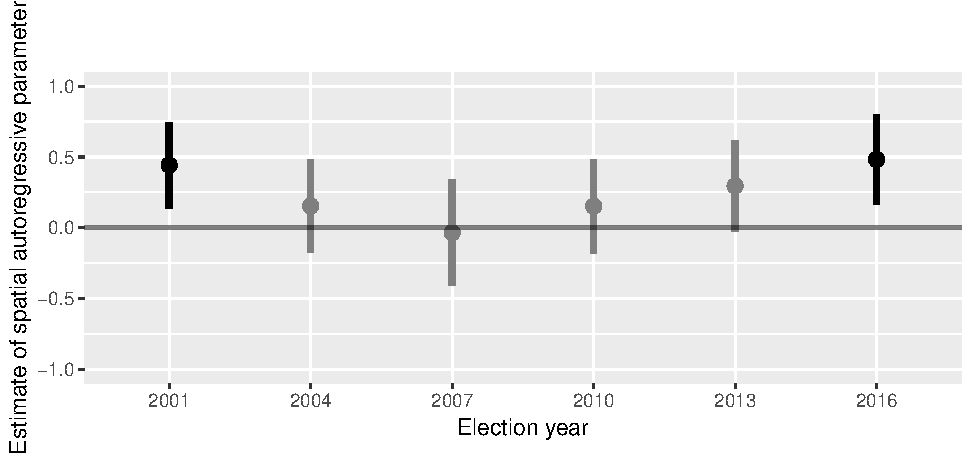
\includegraphics[height=0.15\textheight]{electoral-modelling-draft_files/figure-latex/rhovis-1}

\}

\textbackslash caption\{Estimates of the spatial autoregressive parameter for each of the six elections, with a 95\% confidence interval. Only in 2001 and 2016 is there a significant spatial component.\}\label{fig:rhovis}
\textbackslash end\{figure\}

The spatial autoregressive coefficient \(\rho\) is positive and significant in only the 2001 and 2016 elections, meaning that in these elections, an electorate's political climate was affected by the attitudes of it's neighbours. Conversely, in the other four elections, it appears that after accounting for electoral socio-demographics, there is no significant spatial effect, meaning electorates effectively acted independently.

\hypertarget{influential-socio-demographics}{%
\section{Influential socio-demographics}\label{influential-socio-demographics}}

To investigate the socio-demographics that have a strong effect on the two-party preferred vote, partial residual plots are used. These show the direction, size and significance of an estimated effect - the slope of the prediction line matches the estimated coefficient, and the shaded region represents a 95\% confidence band. If a horizontal line can be drawn through the confidence band, then the effect is insignificant. Plots for each election are faceted to compare the effects over time.

\emph{It is important here to note the ecological fallacy - insights are being drawn at the electorate level, and cannot be inferred for another disaggregate level (e.g.~individual voters).}

\hypertarget{income-and-unemployment}{%
\subsection{Income and unemployment}\label{income-and-unemployment}}

Typically the Labor party campaigns on more progressive policies, which often include tax reform that adversely affects higher income earners, and more generous social assistance programs. Despite this, incomes have only significantly affected the electoral two-party preference in 2016 (see Figure \ref{fig:plotincomes}), with higher income areas associated with support for the Liberal party. In the prior elections, the estimated effect is still positive, albeit insignificant. Unemployment on the other hand, was influential in 2001, 2004 and 2007 elections (Figure \ref{fig:plotunemploy}), with electorates with higher unemployment favouring Labor. This estimated effect has become weaker over time, with unemployment having virtually no effect in 2016.

\begin{figure}[h]

{\centering 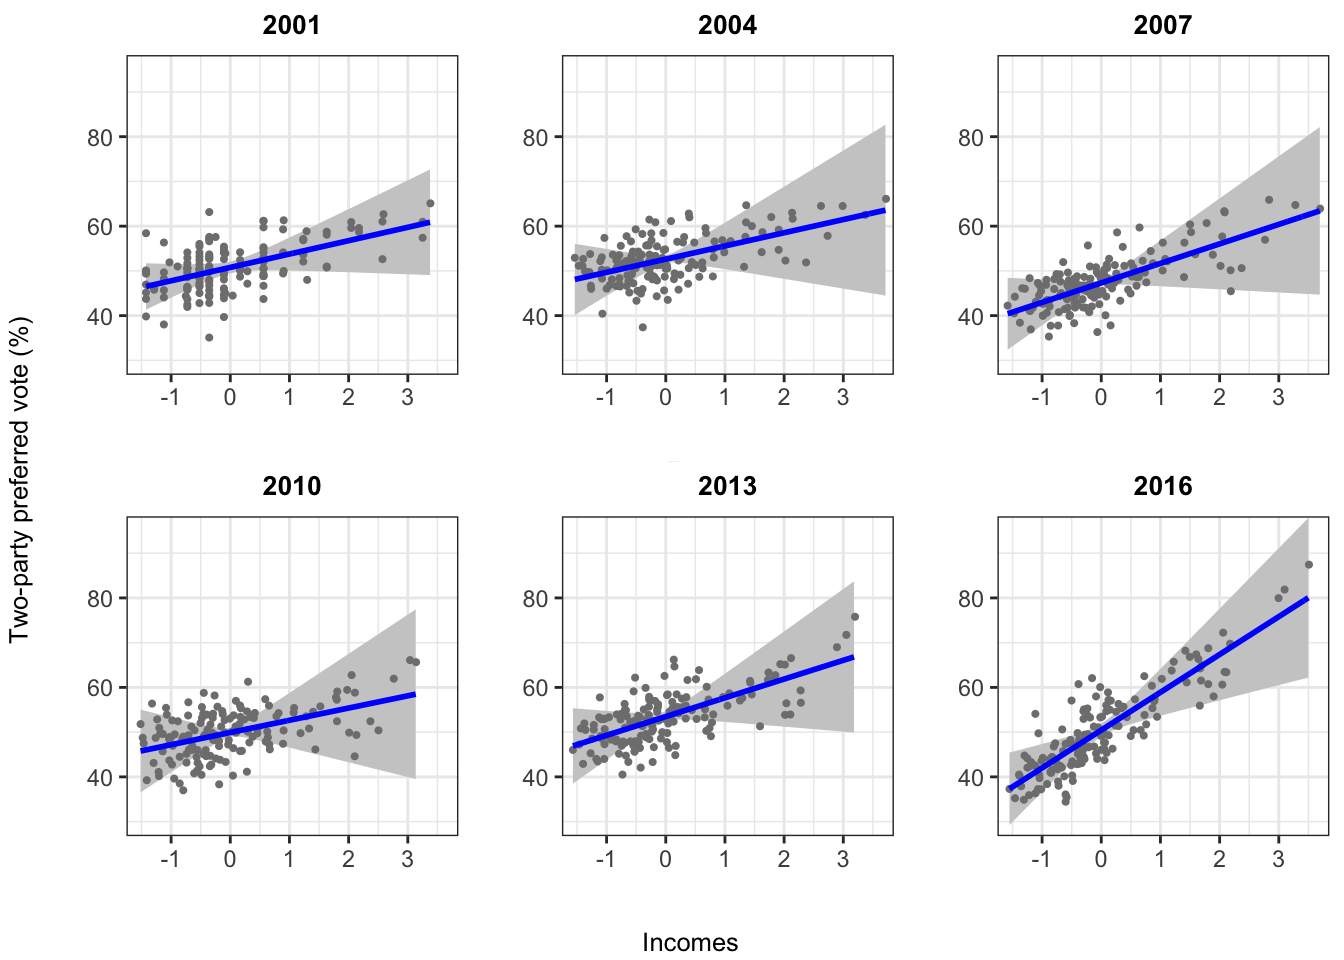
\includegraphics[width=1\linewidth]{electoral-modelling-draft_files/figure-latex/plotincomes-1} 

}

\caption{Effect of Incomes}\label{fig:plotincomes}
\end{figure}

\begin{figure}[h]

{\centering 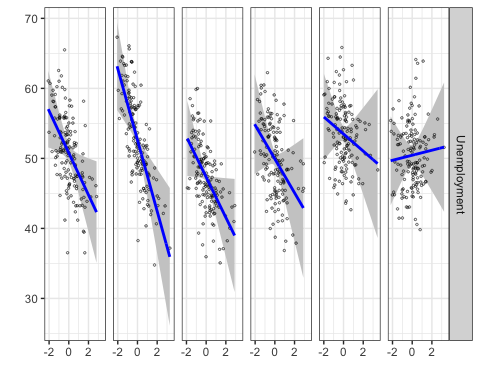
\includegraphics[width=0.6\linewidth]{electoral-modelling-draft_files/figure-latex/plotunemploy-1} 

}

\caption{Effect of Unemployment}\label{fig:plotunemploy}
\end{figure}

\hypertarget{industry-and-type-of-work}{%
\subsection{Industry and type of work}\label{industry-and-type-of-work}}

Electorates with higher proportions of workers in mining, gas, water, agriculture, waste and electricity (grouped as \texttt{Extractive} industries) are consistently linked with higher support for the Liberal party, with the mangitude of this effect slightly increasing over the years (see Figure \ref{fig:plotextractive}). This is unsurprising, as the Liberal party has close ties with these traditional energy industries, and typically present policies to reduce taxation on energy production. Furthermore, electorates with more workers in construction or manufacturing industries (\texttt{Transformative}), as well as wholesale trade, retail trade, transport, post or warehousing (\texttt{Distributive}), are also linked with the Liberal party. However, these effects are not as strong, and \texttt{Transformative} was marginally insignificant in the 2010 election, whereas \texttt{Distributive} was not a key socio-demographic in 2001 or 2016. These effects are shown in Figures \ref{fig:plottransformative} and \ref{fig:plotdistributive}.

\begin{figure}[h]

{\centering 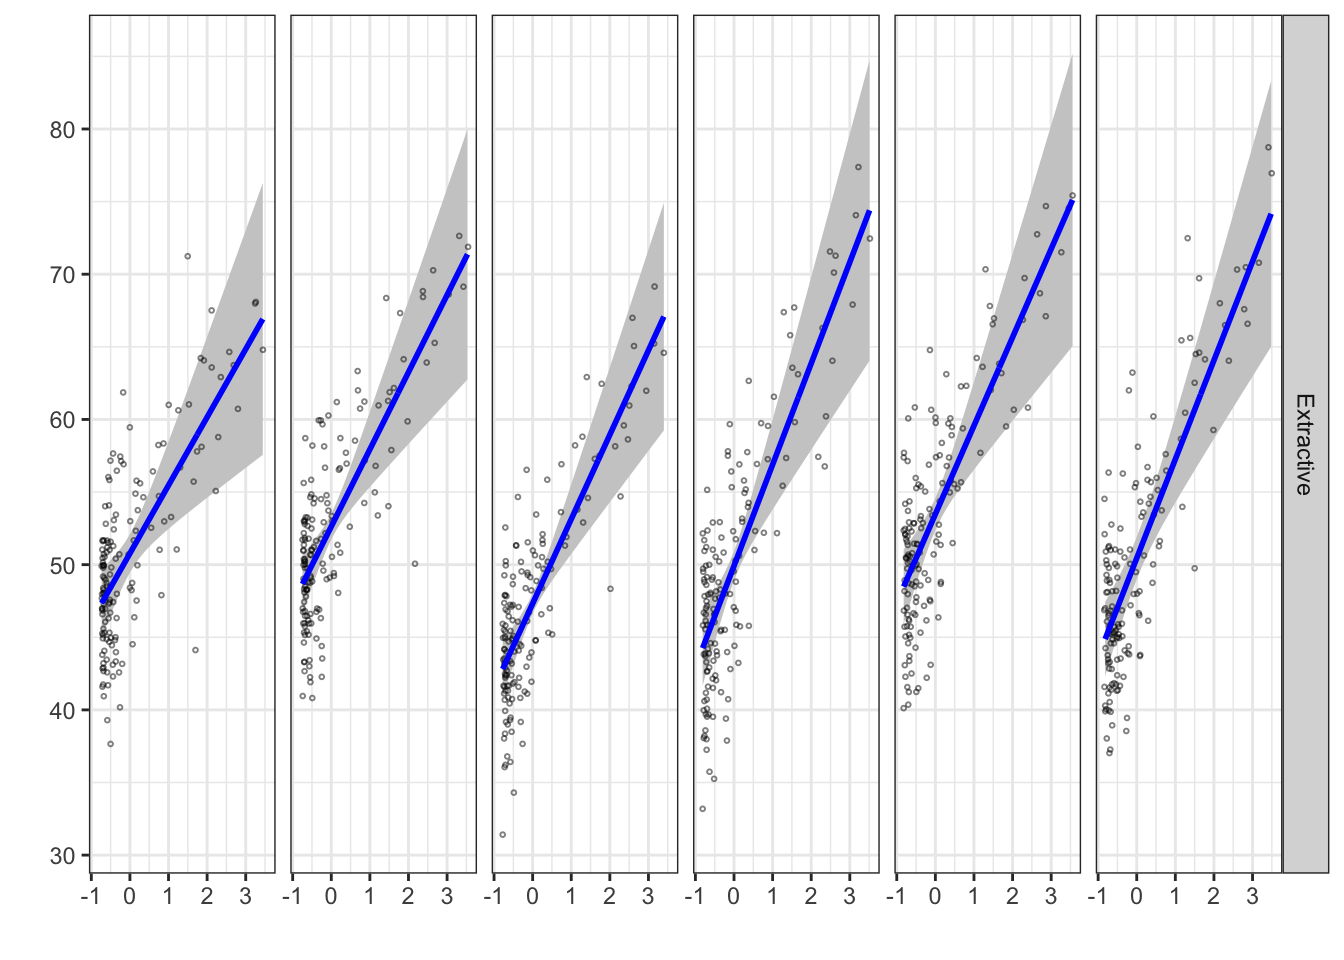
\includegraphics[width=0.6\linewidth]{electoral-modelling-draft_files/figure-latex/plotextractive-1} 

}

\caption{Effect of Extractive}\label{fig:plotextractive}
\end{figure}

\begin{figure}[h]

{\centering 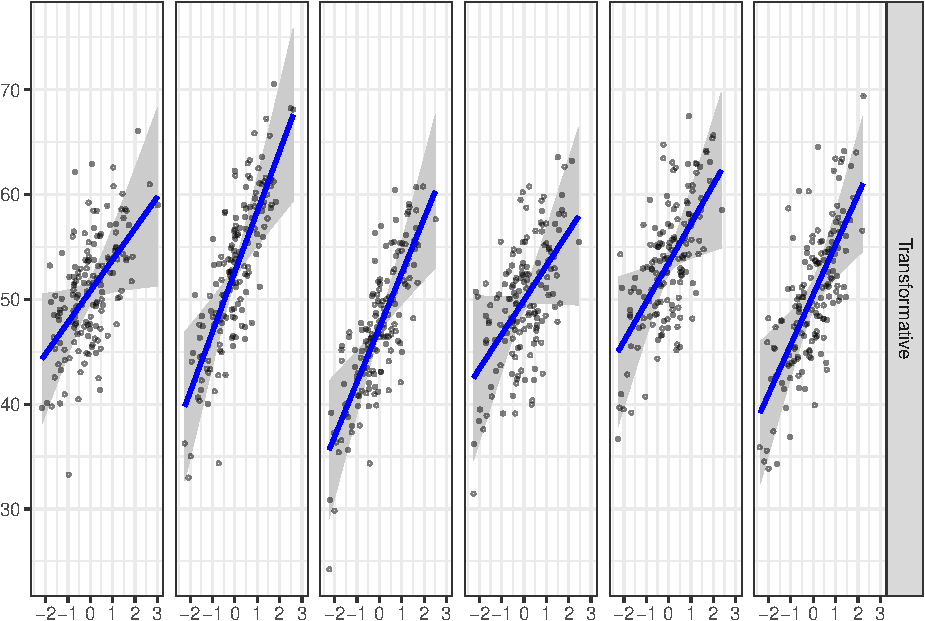
\includegraphics[width=0.6\linewidth]{electoral-modelling-draft_files/figure-latex/plottransformative-1} 

}

\caption{Effect of Transformative}\label{fig:plottransformative}
\end{figure}
\begin{figure}[h]

{\centering 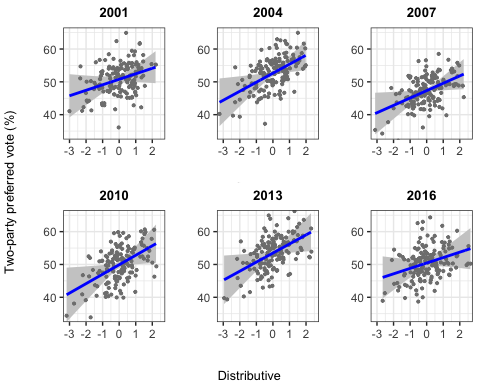
\includegraphics[width=0.6\linewidth]{electoral-modelling-draft_files/figure-latex/plotdistributive-1} 

}

\caption{Effect of Distributive}\label{fig:plotdistributive}
\end{figure}

Similarly, the proportions of workers in managerial, administrative, clerical and sales roles (\texttt{ManagerAdminClericalSales}) is also a significant predictor of two-party preference across all six elections, with higher proportions supporting the Liberal party.

\begin{figure}[h]

{\centering 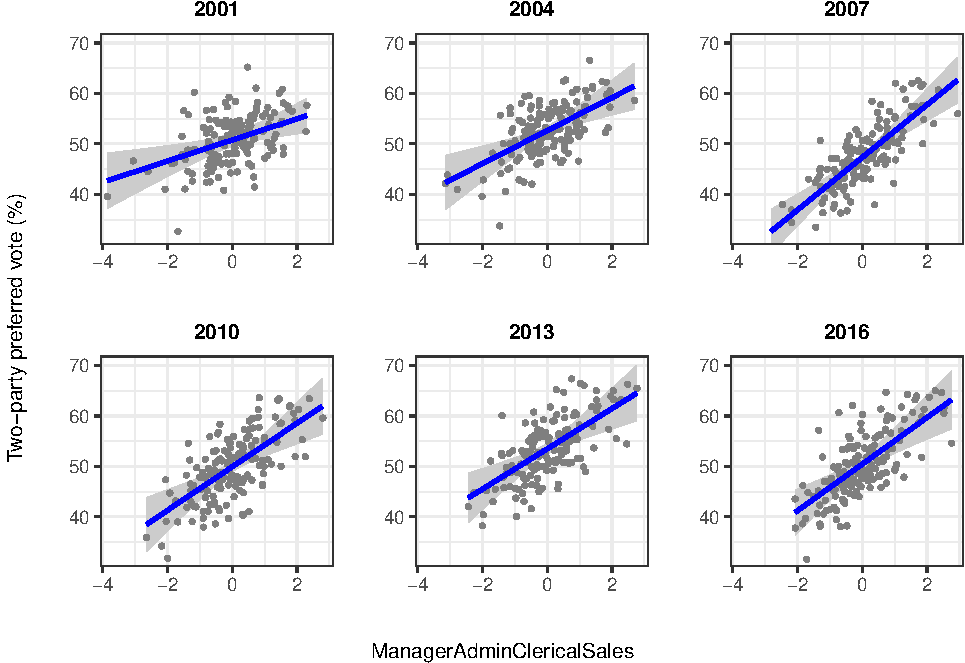
\includegraphics[width=0.6\linewidth]{electoral-modelling-draft_files/figure-latex/plotmanager-1} 

}

\caption{Effect of ManagerAdminClericalSales}\label{fig:plotmanager}
\end{figure}

\hypertarget{household-mobility}{%
\subsection{Household mobility}\label{household-mobility}}

\begin{figure}[h]

{\centering 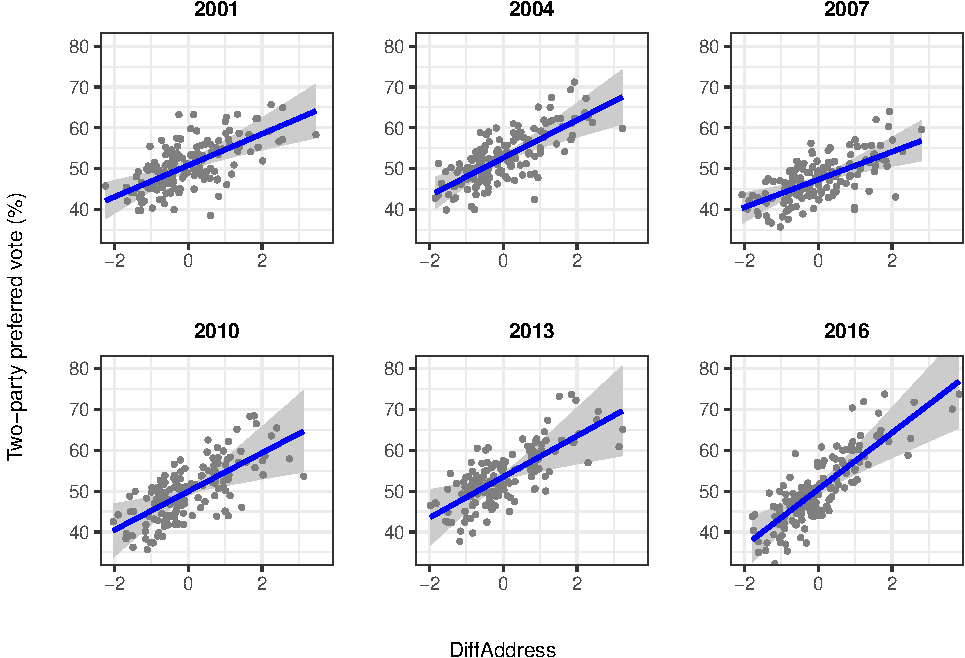
\includegraphics[width=0.6\linewidth]{electoral-modelling-draft_files/figure-latex/plotdiffaddress-1} 

}

\caption{Effect of DiffAddress}\label{fig:plotdiffaddress}
\end{figure}

In each of the six elections, electorates with a higher proportion of people that have recently moved house (meaning in last five years) were more likely to support the Liberal party, with this effect becoming stronger since 2010. Having controlled for characteristics of house ownership and rental prices (via the factors \texttt{PropertyOwned} and \texttt{RentLoan} respectively), this is effect is somewhat surprising. \emph{Add more here?}

\hypertarget{indigenous-population}{%
\subsection{Indigenous population}\label{indigenous-population}}

\begin{figure}[h]

{\centering 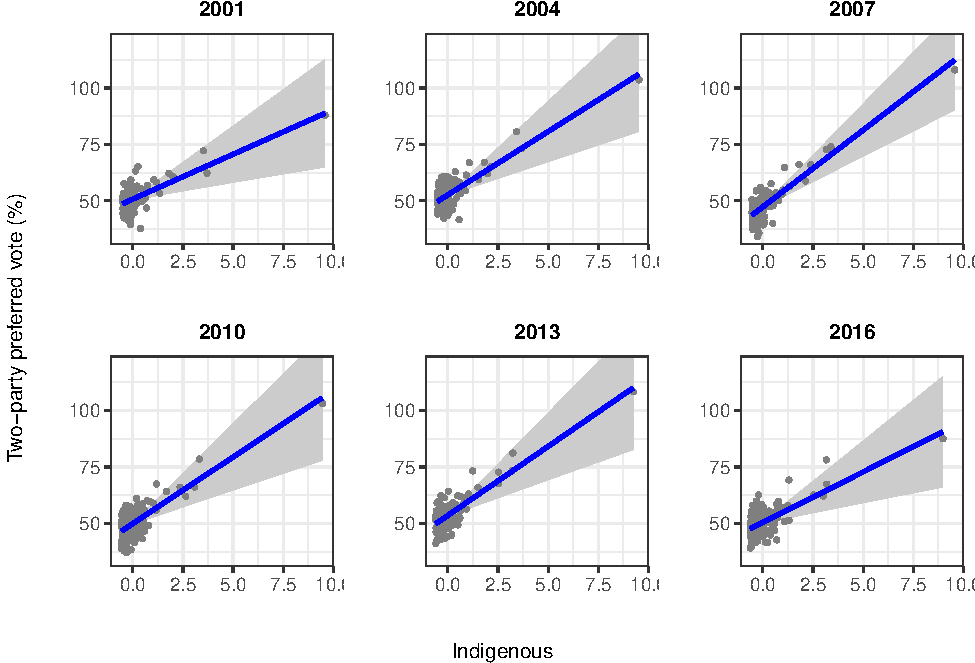
\includegraphics[width=0.6\linewidth]{electoral-modelling-draft_files/figure-latex/plotindigenous-1} 

}

\caption{Effect of Indigenous population}\label{fig:plotindigenous}
\end{figure}

The indigenous population of an electorate is found to be a significant predictor in every election, with higher indigenous populations supporting the Liberal party. There are a few outliers with Lingiari (NT) being the most extreme. However, Lingiari itself has been a strong Labor supporter, and this effect appears to be driven by the other electorates with high Indigenous populations (Kalgoorlie (WA), Leichhardt (NSW), Durack (WA), Parkes(NSW) and Kennedy (QLD)), which have almost always elected a Liberal candidate.

\hypertarget{relationships-and-families}{%
\subsection{Relationships and families}\label{relationships-and-families}}

In each of the six elections, higher proportions people in de facto marriages are tied to support for the Labor party, whereas the effect of marriages themselves are insignificant. Larger family and household size (via the \texttt{FamHouseSize} factor) is also linked with Labor support, although only being significant in the 2007 and 2010 elections (see Figure \ref{fig:plotfamhousesize}).

\hypertarget{a-note-on-similar-variables}{%
\subsection{A note on similar variables}\label{a-note-on-similar-variables}}

Many of the Census variables represent similar information, which is why factors were created and some variables were removed. However, there still remain some variables which are closely related. For example, \texttt{OtherLanguageHome} is the proportion of households that speak a language other than English at home, which is likely to be related to the proportion of people born overseas (a sum of the variables with a \texttt{Born} prefix). In 2001, the coefficient estiamte for \texttt{OtherLanguageHome} is significant and negative, and all \texttt{Born} variables are insignificant. If \texttt{OtherLanguageHome} is removed from the model, populations born in South Eastern Europe (\texttt{Born\_SE\_Europe}) absorb the negative effect (\(p = 0.0011\)).

\hypertarget{a-closer-look-at-the-residuals}{%
\section{A closer look at the residuals}\label{a-closer-look-at-the-residuals}}

\hypertarget{residuals-by-state}{%
\subsection{Residuals by state}\label{residuals-by-state}}

It is often hypothesized that states have systematic differences that cause their electorates to vote differently. Boxplots of residuals grouped by state reveal that only Tasmania and the Australian Capital Territory appear to have a state-specific effect that is not captured by the models. These states appear to have a bias towards Labor. There are few electorates in these states (five and two, respectively), so this might be due to incumbent effects rather than an actual state-specific bias.

\begin{figure}[h]

{\centering 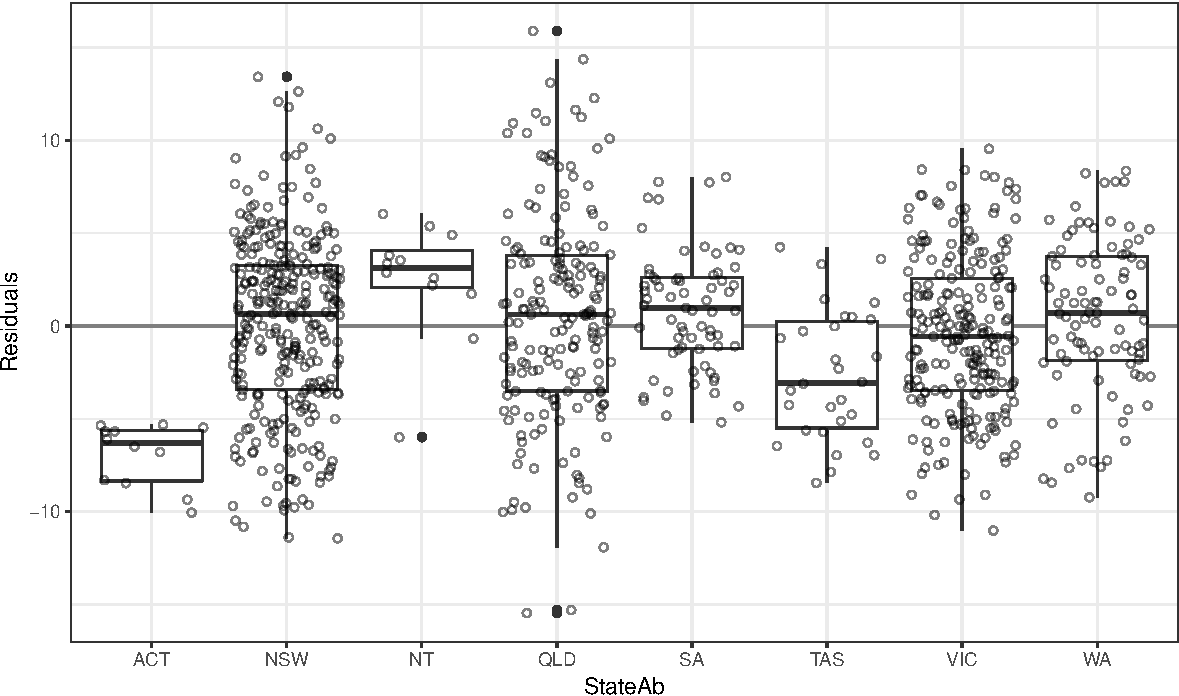
\includegraphics[width=0.75\linewidth]{electoral-modelling-draft_files/figure-latex/resstate-1} 

}

\caption{Boxplot of residuals by state.}\label{fig:resstate}
\end{figure}

\hypertarget{electorates-with-largest-residuals}{%
\subsection{Electorates with largest residuals}\label{electorates-with-largest-residuals}}

The electorates Capricornia (QLD), Leichhardt (QLD) and Riverina (NSW) have the three largest maximum absolute residuals across the six elections. Capricornia is a swing electorate, which strongly supported Labor between 2001 and 2010, before being narrowly won by Liberal in the last two elections. It has many people working in extractive jobs, an above-average Christian population, and above-average proportion of de facto relationships. The model tends to overpredict its two-party preferred vote (in favour of the Liberal party). Leichhardt is an area encompassing the northernmost tip of Queensland and consists of mainly small indigenous communities and uninhabited rural areas, which was won by the Liberal party in all but the 2007 election. It too has an above-average proportion of de facto relationships, along with an above-average proportion of people moving houses and a high proportion of single parent households. The model consistently underpredicts its two-party vote. Riverina is a rural electorate of NSW, and has been a very safe Liberal (National) seat since 1980. It has a relatively monocultural population consisting of a high proportion of Australian citizens and Christians, an above-average amount of extractive jobs and below average education levels. Its Liberal preference is also underpredicted.

\hypertarget{concluding-comments}{%
\chapter{Concluding comments}\label{concluding-comments}}

Across the past six elections, the spatial error models reveal that the electoral socio-demographics driving the two-party preferred vote have remained relatively steady, with industry and type of work being particularly influential, along with the type of relationships and household mobility, among others. The neighbourhood (spatial) effects were only found to be significant in the 2001 and 2016 elections. Surprisingly, unemployment, incomes and family/household sizes were significant in only some elections, and other characteristics like education were not significant at all.

The cross-sectional data set of Census and election data were obtained by collecting information from the ABS and AEC, and then applying a spatio-temporal imputation process, as detailed in section \ref{data}. This data is available in the \texttt{eechidna} \texttt{R} package, which can be downloaded from CRAN. All associated code to produce the data in the package from raw files can be found in the github repository (\url{https://github.com/ropenscilabs/eechidna}), and vignettes on how to use the data are located on the github page (\url{https://ropenscilabs.github.io/eechidna/}).

Furthermore, this paper is generated using the \texttt{knitr} \citep{knitr} package, so code to reproduce the results are contained in the \texttt{RMarkdown} file.

\hypertarget{software}{%
\chapter{Software}\label{software}}

\texttt{eechidna} (Exploring Election and Census Highly Informative Data Nationally for Australia) is an R package that makes it easy to look at the data from the Australian Federal elections and Censuses that occurred between 2001 and 2016. The data in this package includes voting results for each polling booth and electoral division (electorate), Census information for each electorate and maps of the electorates that were in place at the time of each event. All data in this package is obtained from the Australian Electoral Commission, the Australian Bureau of Statistics and the Australian Government. Census data is imputed for the election years in which a Census does not occur via a spatio-temporal imputation method.

The Census and election datasets in the package can be linked by electorate using the unique identifier variable \texttt{UniqueID}. Vignettes describing how to use the data and how the data was obtained, can also be found on \url{https://ropenscilabs.github.io/eechidna/}.

\bibliography{book.bib,packages.bib}


\end{document}
